\chapter{Basic Algorithms}

I will now talk about two very common machine learning algorithms, the boosted decision tree (BDT) and the neural net. Neural nets in particular form the basis of most modern machine learning, and all advanced architectures discussed in this thesis will be some form of neural network.

\section{BDTs}

\subsection*{Decision Tree}

A decision tree is simply a series of cut-based decisions on input data, which one can follow to reach a conclusion. An example of a very simple decision tree is shown in Figure~\ref{decision_tree}.

\begin{figure}[htbp]
    \centering
    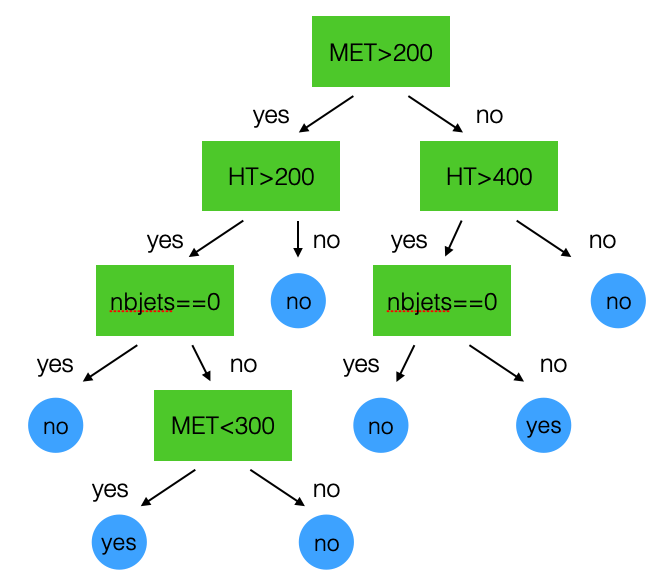
\includegraphics[width=0.5\linewidth]{Images/ML/decision_tree.png}
    \caption{An example of a decision tree used to classify events. Don't read too much into it - I chose the cuts randomly.}
    \label{decision_tree}
\end{figure}

Decision trees work in a similar way to how objects and signal regions are selected in traditional high-energy-physics analyses. For example, one may ask whether an event has more than, less than, or equal to three leptons. If the event has exactly three leptons, one may ask whether the top two leptons have dilepton mass within a certain range, etc. Based on these decisions, an experimenter can decide what signal region an event belongs in. As another example, imagine that we are trying to determine what kind of particle we have seen in an event. We could ask whether the particle left a track in the inner detector, whether the amount of energy it deposited in the calorimeter is in a certain range, etc.
 
A decision tree is usually created by determining what specific single-feature cut will minimize information entropy at each step. The tree is capped at a maximum number of branches or at a maximum depth, in order to prevent overfitting.

An advantage of decision trees is that they are very simple to create and use. Inputs do not have to be numeric, and they don't have to be normalized. Inputs can also have missing values, as long as the tree knows how to classify them. A downside of using a tree is that you have to calculate input features manually, which removes a lot of the benefits of using a machine learning algorithm.

\subsection*{Random Forest}

A random forest operates on a similar principle to a single decision tree. However, now we create multiple trees by sampling a subset of training events for each tree. Each tree in the forest is usually kept pretty shallow, much more so than a single decision tree. A test event is then classified by averaging the results of all trees in the forest.

\subsection*{Boosted Decision Tree}

A boosted decision tree is also created by combining many different decision trees together, but the training is performed in a more complex way. Like the random forest, any individual tree in the BDT can be very weak, containing only a small number of branches and a small maximum depth. However, by using a boosting algorithm such as AdaBoost, these weak learners can be combined into an effective classification algorithm.

The way that AdaBoost works is by assigning an initial uniform weight $D_1(i)$ to each event $i$ in the training data. At each time step $t$ we train a new tree on the data with event weights $D_t$, then give the tree a grade $\epsilon_t$ based on its event-weighted error. A learning rate is calculated, based on the performance of the tree:

\begin{align}
    \alpha_t &= \frac{1}{2}\ln{\frac{1-\epsilon_t}{\epsilon_t}}
\end{align}

This learning rate is positive when the tree performs well (error below $0.5$), and negative otherwise. The event weights are then updated based on the learning rate $\alpha_t$, and whether or not the tree classified each event properly. In the following equation, the tree's output for event $x_i$ is $h_t(x_i)$, the true classification is $y_i$, and $Z_t$ is a normalization factor:

\begin{align}
    D_{t+1}(i) &= \frac{D_t(i)\exp(-\alpha_t y_i h_t(x_i))}{Z_t}
\end{align}

At the end of training, we can now classify a test event by the weighted sum of all trees obtained during the training procedure:

\begin{align}
    H(x) &= \text{sign}(\sum_{t=1}^T \alpha_t h_t(x))
\end{align}

\section{Neural Nets}

A neural net is a machine learning algorithm based on the physical structure of neurons in an organic brain. The basic unit is a neuron, which has a numerical value and is connected by weighted dendrites to any number of input neurons and any number of output neurons.

A simple example net is show in Figure~\ref{fig:neural_net}. For each event, numerical inputs are set on the first layer of the neural net, and the values of resulting neurons are calculated based on their connections and weights. Neuron values on the final layer of the net are taken as outputs. All layers in between are referred to as hidden layers.

\begin{figure}[htbp]
    \centering
    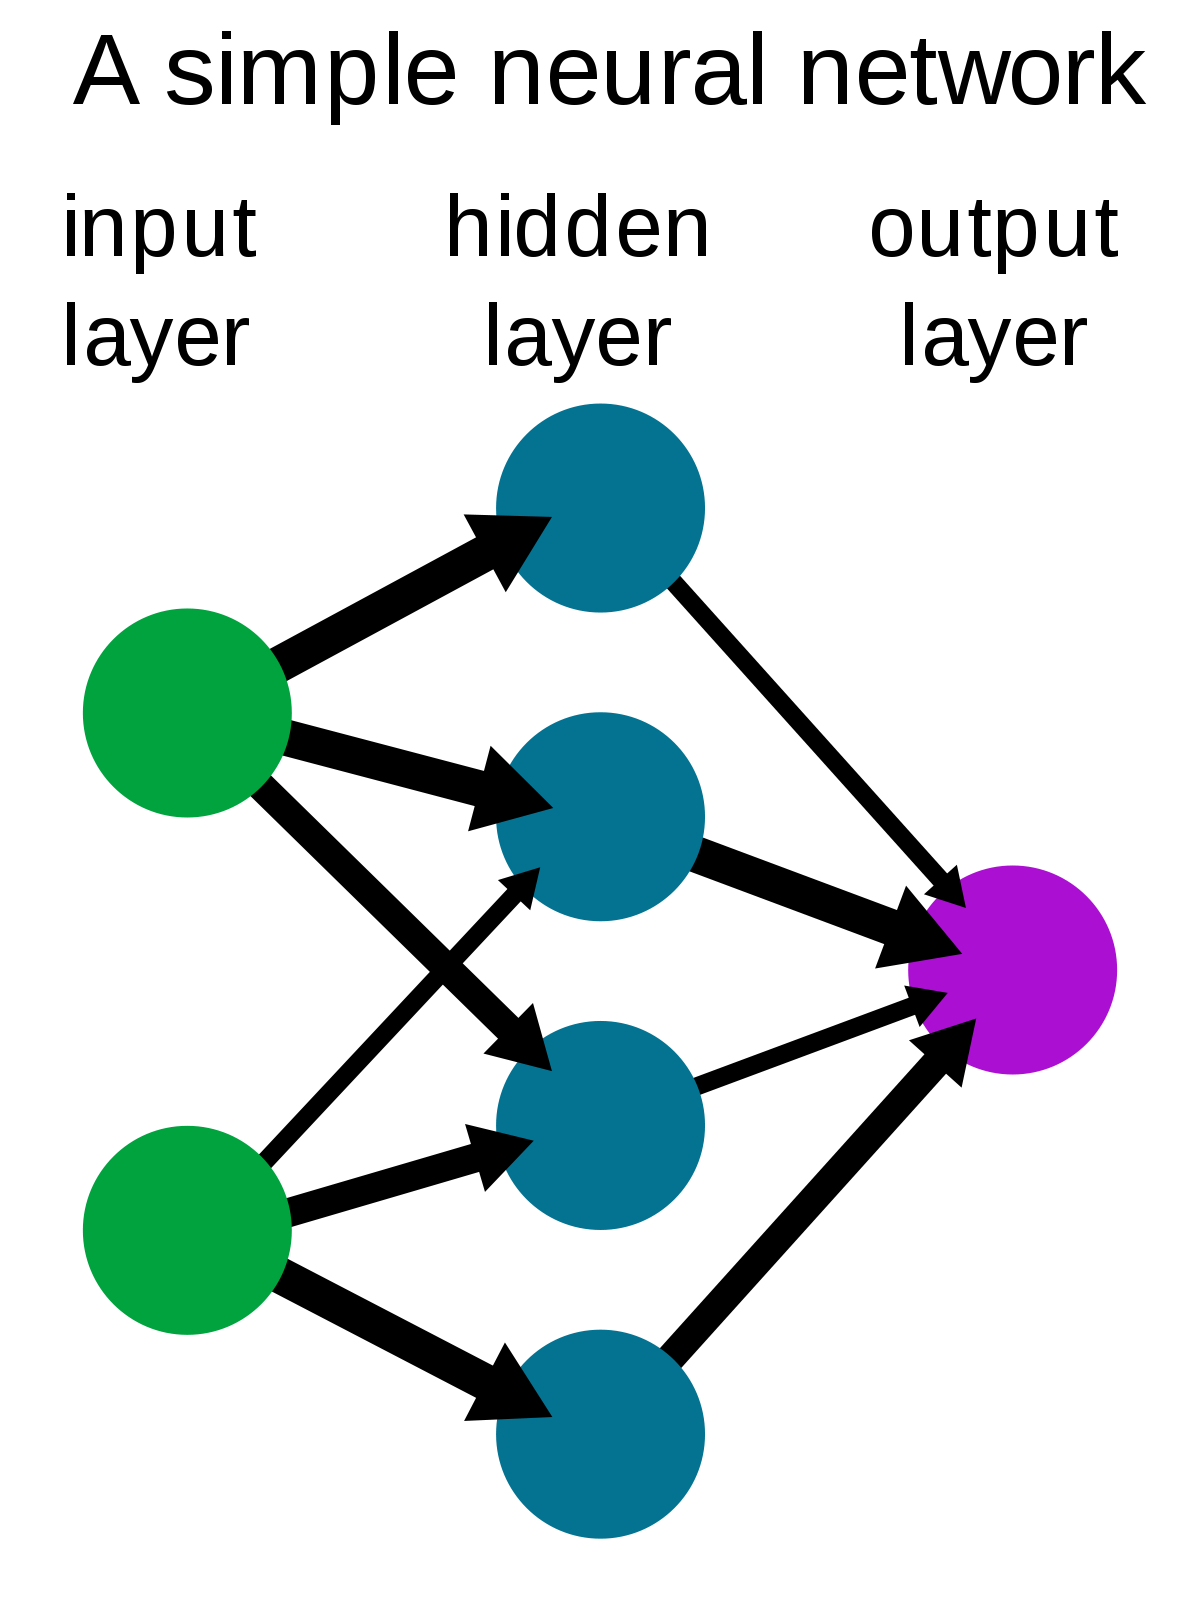
\includegraphics[width=0.3\linewidth]{Images/ML/neural_net.png}
    \caption{A diagram showing a typical densely-connected neural net.}
    \label{fig:neural_net}
\end{figure}

The value of each neuron is determined by the values of neurons that feed into it, along with their inter-neural connection weights. Each neuron also has a bias value. Finally, a neuron typically has an associated "activation function", which is usually the tanh or sigmoid function, and which will be discussed later. Overall, the total value $v$ of a neuron, as determined by its $n$ connecting neurons, bias value $b$, weights between neurons $W$, and activation function $\sigma$, is given by:

\begin{align}
    v_i &= \sigma \left( \sum_{j=0}^n W_{j\rightarrow i} v_j + b_i \right)
\end{align}

For now we will only consider simple feed-forward neural nets, where all the inputs to a neuron come from the previous layer, and all the outputs of that neuron go to the next layer. That is, there are no "loops", and there are no connections between neurons on the same layer. If we consider $W$ as a weight matrix between layers of neurons, we can say that the values of all neurons on layer $i$ are equal to:

\begin{align}
    \Vec{v}_i &= \sigma(W \Vec{v}_{i-1} + \Vec{b}_i)
\end{align}

\subsection*{Activation Functions}

The purpose of the nonlinear activation function on each neuron is two-fold. First, the non-linearity of the function makes a multi-layer net not simply a combination of linear functions, which is itself a linear function. Rather, with the activation functions included, a large enough neural net becomes a universal function approximator. Second, the activation function causes a neuron's value to lie within a set range, usually below an absolute value of 1. This prevents net values from exploding over multiple layers.

\subsection*{Training via Gradient Descent}

In order to train a neural net, we use "gradient descent with back-propagation", meaning that for each input (or batch of inputs) we calculate the derivative of the loss function with respect to every weight and bias value in the net. Using these numbers, we perform gradient descent by updating each weight and bias in proportion to its gradient and a set learning rate, commonly denoted $\alpha$. The training occurs over many input events, with loss gradually decreasing and accuracy gradually increasing. Essentially, the neural net training via gradient descent is simply conducting computational function optimization on the loss. Back-propagation refers to the specific computational method used to calculate gradients, and will not be discussed here.

\section{Basic Training Concepts}

\subsection*{Overfitting, Underfitting, and Testing}

Any sufficiently general function can be made to fit any arbitrary distribution simply by making it more complex. For example, a polynomial function may be made to fit any 2D data by making the polynomial the same order as the number of data points. However, this function would be crazy looking and would not generalize well to new data points. In other words, it would not be a good predictive algorithm.

On the other hand, a very simple function such as a first-order polynomial (a straight line) would also not be a good predictor for most distributions. Such a simple function would also achieve low accuracy (and a high loss) on the training data.

Here we have described the problem of underfitting vs. overfitting a distribution. An underfit function does not describe the training data well, but an overfit function describes it too well, and does not generalize. The best solution is one which describes the training data adequately, but does not become unnecessarily complex.

Since neural nets are universal function approximators, we have to make sure that we end training before overfitting occurs. In order to monitor the training status of our net, we usually split our data into a training set and a test set. We apply gradient descent using the training data, but every once in a while we evaluate performance on the test data as well. Ideally, loss should decrease for both training and test data. If loss continues to decrease for training data, but begins to increase for test data, then the model has lost generalizeability and has become overtrained.

\subsection*{Regularization and Dropout Layers}

To prevent overtraining, we can use a class of methods known as regularization. Essentially, these methods put some kind of constraint on the net such that it is disincentivized against overfitting. A common method is to add a regularization term to the loss function which is simply equal to the L2 sum of all weights and biases in the net. This incentivizes the net to keep things simple.

Another commonly used method is to include dropout layers within the net. What these layers do is simply turn off inputs from the previous layer with some probability. So for example, a dropout layer with a passing probability of 80\% will on average zero out 20\% of the neurons on the previous layer during each training pass. This is another way of forcing the net to keep things simple, and to not rely on large weights balancing each other out. It also forces the net to examine all parts of the input data, and not rely solely on a single component. During actual usage of the net, dropout layers are turned off.

\section{ML Software}

There are multiple machine learning software packages for Python. Some of the best-known ones are scikit-learn, TensorFlow, and PyTorch.

Scikit-learn contains non-neural algorithms, such as boosted decision trees, support vector machines, and unsupervised algorithms such as k-nearest neighbor and k-means. It also contains basic functionality for calculating things like accuracy, area-under-curve for a ROC curve, etc. It's a very useful general toolkit.

PyTorch and TensorFlow are two competing packages specialized for dealing with neural nets. PyTorch was created by Facebook, and TensorFlow was created by Google. A big chunk of what makes these packages great are their support for automatic differentiation. In other words, you can build up your models in these frameworks by defining neural layers and the connections between them. You then specify which parameters need to be trained, and which should be held fixed. Then you can pass in an input, calculate a loss value, and automatically differentiate the loss with respect to every trainable parameter in the model. Many common neural architectures are built into the packages, and you can even load pre-trained nets for some common types of problems. Both packages also offer support for many types of gradient descent and learning rate optimization algorithms. The GPU support is also very good and easy to use for both packages.

For the machine learning projects described in this thesis, we first began by using TensorFlow, but due to PyTorch's improved support for non-static graphs at the time, we soon began using PyTorch exclusively. By non-static graphs, I mean that with PyTorch you could pause computation in the middle of a net and look at net states, and even change the architecture if you wanted to, which made PyTorch very useful for development and debugging. This difference has since disappeared with the introduction of TensorFlow 2.0, which now includes support for dynamic graphs.

\section{Other Topics}

Different arrangements of neurons and connections are referred to as "architectures". A basic net composed of layers of neurons, where every neuron in one layer is connected to every neuron in the following layer, is called a dense neural net (DNN) or a fully-connected net, but we will discuss more complex architectures in the next chapter.

Many other important topics, such as weight initialization, learning rate optimization and methods of gradient descent, pooling and batch normalization, hyperparameter optimization algorithms etc. will not be discussed in this review due to space and scope constraints.